%% Creator: Inkscape inkscape 0.92.4, www.inkscape.org
%% PDF/EPS/PS + LaTeX output extension by Johan Engelen, 2010
%% Accompanies image file 'Beispielgrafik.pdf' (pdf, eps, ps)
%%
%% To include the image in your LaTeX document, write
%%   \input{<filename>.pdf_tex}
%%  instead of
%%   \includegraphics{<filename>.pdf}
%% To scale the image, write
%%   \def\svgwidth{<desired width>}
%%   \input{<filename>.pdf_tex}
%%  instead of
%%   \includegraphics[width=<desired width>]{<filename>.pdf}
%%
%% Images with a different path to the parent latex file can
%% be accessed with the `import' package (which may need to be
%% installed) using
%%   \usepackage{import}
%% in the preamble, and then including the image with
%%   \import{<path to file>}{<filename>.pdf_tex}
%% Alternatively, one can specify
%%   \graphicspath{{<path to file>/}}
%% 
%% For more information, please see info/svg-inkscape on CTAN:
%%   http://tug.ctan.org/tex-archive/info/svg-inkscape
%%
\begingroup%
  \makeatletter%
  \providecommand\color[2][]{%
    \errmessage{(Inkscape) Color is used for the text in Inkscape, but the package 'color.sty' is not loaded}%
    \renewcommand\color[2][]{}%
  }%
  \providecommand\transparent[1]{%
    \errmessage{(Inkscape) Transparency is used (non-zero) for the text in Inkscape, but the package 'transparent.sty' is not loaded}%
    \renewcommand\transparent[1]{}%
  }%
  \providecommand\rotatebox[2]{#2}%
  \newcommand*\fsize{\dimexpr\f@size pt\relax}%
  \newcommand*\lineheight[1]{\fontsize{\fsize}{#1\fsize}\selectfont}%
  \ifx\svgwidth\undefined%
    \setlength{\unitlength}{265.58093262bp}%
    \ifx\svgscale\undefined%
      \relax%
    \else%
      \setlength{\unitlength}{\unitlength * \real{\svgscale}}%
    \fi%
  \else%
    \setlength{\unitlength}{\svgwidth}%
  \fi%
  \global\let\svgwidth\undefined%
  \global\let\svgscale\undefined%
  \makeatother%
  \begin{picture}(1,1.05335122)%
    \lineheight{1}%
    \setlength\tabcolsep{0pt}%
	\fontseries{md}\fontshape{n}\selectfont
	\footnotesize
    \put(0,0){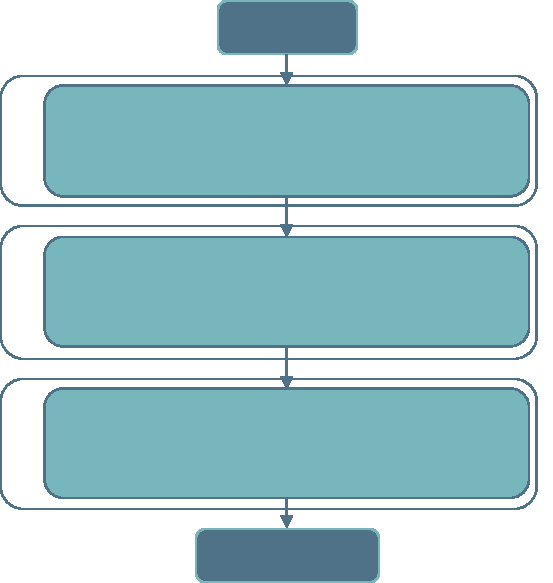
\includegraphics[width=\unitlength,page=1]{Kap_2/Grafiken/Beispielgrafik.pdf}}%
	\put(0.52,0.99404727){\color{rptugruengrau}\makebox(0,0)[ct]{\lineheight{1.25}\smash{\begin{tabular}[t]{c}Start\end{tabular}}}}%
	\put(0.52,0.038){\color{rptugruengrau}\makebox(0,0)[ct]{\lineheight{1.25}\smash{\begin{tabular}[t]{c}Ende\end{tabular}}}}%
	
	\scriptsize
    \put(0.05072458,0.745){\color{rptublaugrau}\rotatebox{90}{\makebox(0,0)[lt]{\lineheight{1.25}\smash{\begin{tabular}[t]{l}Schritt 1\end{tabular}}}}}%
	\put(0.05072458,0.47){\color{rptublaugrau}\rotatebox{90}{\makebox(0,0)[lt]{\lineheight{1.25}\smash{\begin{tabular}[t]{l}Schritt 2\end{tabular}}}}}%
	\put(0.05072458,0.19){\color{rptublaugrau}\rotatebox{90}{\makebox(0,0)[lt]{\lineheight{1.25}\smash{\begin{tabular}[t]{l}Schritt 3\end{tabular}}}}}%
    
	\fontsize{7.5}{7.5}
    \put(0.1,0.83872738){\color{rptublaugrau}\makebox(0,0)[lt]{\lineheight{1.25}\smash{\begin{tabular}[t]{l}•\end{tabular}}}}%
    \put(0.12,0.83872738){\color{rptublaugrau}\makebox(0,0)[lt]{\lineheight{1.25}\smash{\begin{tabular}[t]{l}Dies ist eine Beispielgrafik,\end{tabular}}}}%
    \put(0.1,0.8076634){\color{rptublaugrau}\makebox(0,0)[lt]{\lineheight{1.25}\smash{\begin{tabular}[t]{l}•\end{tabular}}}}%
    \put(0.12,0.8076634){\color{rptublaugrau}\makebox(0,0)[lt]{\lineheight{1.25}\smash{\begin{tabular}[t]{l}die zeigen soll, wie eine pdf Grafik inkl. Text\end{tabular}}}}%
    \put(0.1,0.77659943){\color{rptublaugrau}\makebox(0,0)[lt]{\lineheight{1.25}\smash{\begin{tabular}[t]{l}•\end{tabular}}}}%
    \put(0.12,0.77659943){\color{rptublaugrau}\makebox(0,0)[lt]{\lineheight{1.25}\smash{\begin{tabular}[t]{l}in \LaTeX \ eingebettet werden kann\end{tabular}}}}%
    \put(0.1,0.74553545){\color{rptublaugrau}\makebox(0,0)[lt]{\lineheight{1.25}\smash{\begin{tabular}[t]{l}•\end{tabular}}}}%
    \put(0.12,0.74553545){\color{rptublaugrau}\makebox(0,0)[lt]{\lineheight{1.25}\smash{\begin{tabular}[t]{l}Dabei lässt sich nicht nur die Schrift anpassen\end{tabular}}}}%
    \put(0.1,0.56479958){\color{rptublaugrau}\makebox(0,0)[lt]{\lineheight{1.25}\smash{\begin{tabular}[t]{l}•\end{tabular}}}}%
    \put(0.12,0.56479958){\color{rptublaugrau}\makebox(0,0)[lt]{\lineheight{1.25}\smash{\begin{tabular}[t]{l}Auch die Schriftfarbe,\end{tabular}}}}%
    \put(0.1,0.53373561){\color{rptublaugrau}\makebox(0,0)[lt]{\lineheight{1.25}\smash{\begin{tabular}[t]{l}•\end{tabular}}}}%
    \put(0.12,0.53373561){\color{rptublaugrau}\makebox(0,0)[lt]{\lineheight{1.25}\smash{\begin{tabular}[t]{l}die Schriftgröße,\end{tabular}}}}%
    \put(0.1,0.50267163){\color{rptublaugrau}\makebox(0,0)[lt]{\lineheight{1.25}\smash{\begin{tabular}[t]{l}•\end{tabular}}}}%
    \put(0.12,0.50267163){\color{rptublaugrau}\makebox(0,0)[lt]{\lineheight{1.25}\smash{\begin{tabular}[t]{l}Schriftart\end{tabular}}}}%
    \put(0.1,0.47160765){\color{rptublaugrau}\makebox(0,0)[lt]{\lineheight{1.25}\smash{\begin{tabular}[t]{l}•\end{tabular}}}}%
    \put(0.12,0.47160765){\color{rptublaugrau}\makebox(0,0)[lt]{\lineheight{1.25}\smash{\begin{tabular}[t]{l} und Schriftposition lässt sich anpassen\end{tabular}}}}%
    \put(0.1,0.2767518){\color{rptublaugrau}\makebox(0,0)[lt]{\lineheight{1.25}\smash{\begin{tabular}[t]{l}•\end{tabular}}}}%
    \put(0.12,0.2767518){\color{rptublaugrau}\makebox(0,0)[lt]{\lineheight{1.25}\smash{\begin{tabular}[t]{l}Die Schriftposition wird\end{tabular}}}}%
    \put(0.1,0.24568782){\color{rptublaugrau}\makebox(0,0)[lt]{\lineheight{1.25}\smash{\begin{tabular}[t]{l}•\end{tabular}}}}%
    \put(0.12,0.24568782){\color{rptublaugrau}\makebox(0,0)[lt]{\lineheight{1.25}\smash{\begin{tabular}[t]{l}über Koordinaten eingestellt\end{tabular}}}}%
    \put(0.1,0.21462384){\color{rptublaugrau}\makebox(0,0)[lt]{\lineheight{1.25}\smash{\begin{tabular}[t]{l}•\end{tabular}}}}%
    \put(0.12,0.21462384){\color{rptublaugrau}\makebox(0,0)[lt]{\lineheight{1.25}\smash{\begin{tabular}[t]{l}die Farben über den \texttt{color} Befehl\end{tabular}}}}%

  \end{picture}%
\endgroup%
